% !TEX root = domain_transduction.tex
We evaluate our algorithm on various unsupervised domain adaptation tasks while focusing on two different problems, hand-written digit classification and object recognition. For each experiment, we use three domains and extensively evaluate all transfer scenarios.

\begin{table*}[ht]
\caption{Accuracy of our method and the state-of-the-art algorithms on Office dataset and various adaptation settings}
\label{tab:res}
\begin{sc}
\begin{center}
\begin{small}
\begin{tabular}{@{}rcccccc@{}} \toprule 
 Source & Amazon & D-SLR & Webcam & Webcam &Amazon & D-SLR \\
 Target & Webcam & Webcam & D-SLR & Amazon & D-SLR & Amazon \\
 \midrule
GFK \cite{gong2012} & $.398$ & $.791$ & $.746 $ & $.371$ & $.379$ & .379   \\
SA* \cite{fernando13} & $.450$ & $.648$ & $.699$ & $.393$ & $.388$ & $.420$ \\
DLID \cite{chopra13} & $.519$ & $.782$ & $.899$ & -&- &- \\
DDC \cite{tzeng14} & $.618$ & $.950$ & $.985$ & $.522$ & $.644$& $.521$\\
DAN \cite{wang15} & $.685$ & $.960$ & $.990$ & $.531$ & $.670$ & $.540$ \\
Backprop \cite{ganin15} & $.730$ &$\mathbf{.964}$ & $\mathbf{.992}$ & $.536$ & $.728$ & $.544$\\
\midrule
Source Only & $.642$ & $.961$ & $.978$ & $.452$ & $.668$ & $.476$ \\
Our Method & $\mathbf{.804}$ &.962 & $.989$ & $\mathbf{.625}$ & $\mathbf{.839}$ & $\mathbf{.567}$ \\
 \bottomrule
\end{tabular}
\end{small}
\end{center}
\end{sc}
\end{table*}

\begin{table}[ht]
\caption{Accuracy of our method and the digit classification task.}
\label{tab:res2}
\begin{sc}
\begin{small}
\resizebox{\columnwidth}{!}{%
\begin{tabular}{@{}r@{\hskip 1mm}c@{\hskip 1mm}c@{\hskip 1mm}c@{\hskip 1mm}c@{}} \toprule 
Source & M-M & MNIST  & SVHN & MNIST \\
Target&  MNIST & M-M & MNIST & SVHN\\
 \midrule
SA* \cite{fernando13}&  & $.569$ & $.593$ & \\
BP \cite{ganin15} &$.732$ & $.766$ & $.738$ & $.289$ \\
\midrule
Source Only  & $.483$ & $.522$  &.549 &\\
Our Method & $\mathbf{.835}$ & $\mathbf{.855}$ & $\mathbf{.774}$ & $\mathbf{.323}$\\
 \bottomrule
\end{tabular}}
\end{small}
\end{sc}
\end{table}
\subsection{Dataset}
In order to experiment our algorithm on the task of digit classification, we use MNIST\cite{mnist}, Street View House Number\cite{svhn} and artificailly generated version of MNIST, MNIST-M\cite{ganin15}. MNIST is the collection of 60k handwritten digits. For MNIST-M, we generate a series of digit images by using the original MNIST dataset and the color images of BSDS500\cite{bsds500} following the method explained in \cite{ganin15}. Since the dataset is not distributed directly by the authors, we further confirmed that the performance is similar to experimented in \cite{ganin15}. Street view house numbers dataset is a collection of house numbers collected directly from Google street view images. Among many important differences exist between these domains, most significant ones are MNIST being grayscale and the others being colored, SVHN images having extra confusing digits around the centered digit of interest. Moreover, all three of these domains are large-scale having at least 60k examples over 10 classes. 

On the other hand, we use Office\cite{office} dataset in order to evaluate our algorithm on the task of object recognition. Office dataset includes images of the same objects taken directly from Amazon, captured with a cheap webcam and captured with a D-SLR camera. Notable differences of these domains include the white background of Amazon images vs realistic backgrounds of webcam and D-SLR images, and the resolution difference of webcam and D-SLR. Office dataset have rather fewer number of images as maximum 2478 images per domain. On the other hand, it has larger number of classes since there are 31 object categories.

\subsection{Baselines}
We compare our method with variety of algorithms both using and not using feature learning. Considering the two different lines of work, \textbf{SA*}\cite{fernando13} is the dominant state-of-the-art approach not employing any feature learning on other hand \textbf{Backprop(BP)}\cite{ganin15} is the dominant state-of-the-art approach employing feature learning. We use the available source code of \cite{ganin15} and \cite{fernando13} and following the evaluation procedure in \cite{fernando13}, we choose the hyper-parameter of \cite{fernando13} as the highest performing one among various alternatives. In addition to the baselines, we also compare our method with various self-baselines. The most important one is the \textbf{source only} baseline which is a convolutional neural network trained only using the source code. In other words, we only add a softmax layer on top of the features. This is clearly different from our classifier -nearest neighbor-; however, we experimentally validated that softmax always outperformed nearest neighbor based classifier. Hence, we use the highest performing source only method in our results.

\subsection{Implementation Details}
\label{imp_det}
Although our algorithm have very few design parameters and we decide most of them either using cross-validation or exhaustive grid search, our algorithm uses an existing differentiable feature function. The selection of this feature function is a critical parameter for our algorithm. Following the unparalleled success of convolutional neural networks (CNNs), we use CNNs as our feature functions.  In order to have  fair comparison with existing algorithms, we follow the same architecture used by \cite{ganin15}. We only change the feature dimensionality and experiment on the effect of feature dimension. Hence, we use the following architectures for domains \emph{(see supplementary material for full details)}:

\noindent \textbf{MNIST, MNIST-M} and \textbf{SVHN:} Modified LeNet\cite{lenet} as;


\includegraphics[width=\columnwidth]{lenet}


\noindent \textbf{Office:} Modified AlexNet\cite{alexnet} as;

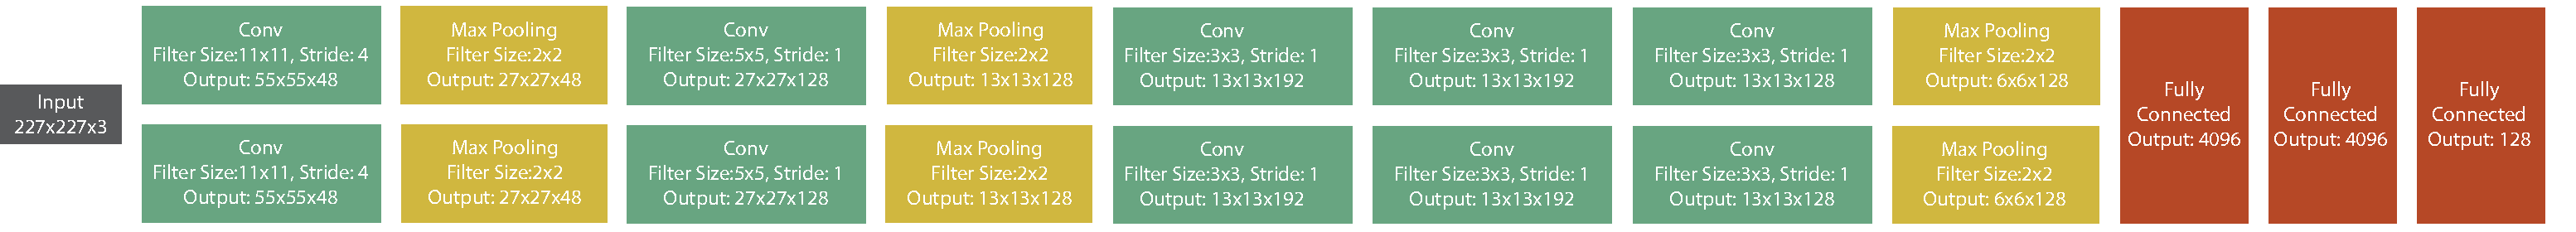
\includegraphics[width=\columnwidth]{alexnet}


where \textbf{C} is convolution, \textbf{P} is max-pooling, \textbf{R} is ReLU and \textbf{F} is fully connected layer. 

Since the office dataset is quite small, we do not learn the full network for office experiments instead we only optimize for fully connected layers initializing with the weights  pre-trained on ImageNet. Moreover, in all of our experiments we set the feature dimension as $128$. We use stochastic gradient descent in order to learn the feature function as well as the similarity metric with AdaGrad\cite{adagrad}. We initialize all variables with truncated normals having unit variance and use the learning rate $2.5x10^{-4}$ and the batch size $256$. 



We further share our learned models as well as the source code using TensorFlow\cite{tensorflow} on \url{http://anonymous.xyz}


\subsection{Evaluation Procedure}
We use the standard evaluation setup of \cite{office}. In other words, we evaluate all algorithms in fully transductive setup. We feed training images and labels of the first domain as the source and feed training images of the second domain as the target. We further evaluate the accuracy on the target domain labels as the ratio of correctly labeled images to all target images. In order to evaluate our algorithm fairly, we first use cross-validation to decide on the margin $\alpha$ and label propagation tradeoff $\lambda$. 


\subsection{Results}

Following the fully transductive evaluation, we summarize the results in Table~\ref{tab:res} and Table~\ref{tab:res2}. Table~\ref{tab:res} summarizes the experimental results on the object recognition experiment using office dataset whereas  table~\ref{tab:res2} summarizes the digit classification experiments on MNIST and SVHN.

Table~\ref{tab:res} suggests that our algorithm is on-par with the state of the art methods for D-SLR$\leftrightarrow$Webcam experiments. This is rather expected since the domain difference is very minor between D-SLR and webcam images. This very minor domain difference results in early saturation of accuracies for all algorithms. Moreover, since we use nearest neighbor classifier, our algorithm needs a large-dataset to be successful. Both webcam and D-SLR datasets are rather small (300to700 examples) which limits the accuracy of nearest neighbor algorithm as well.

\begin{figure}[ht]
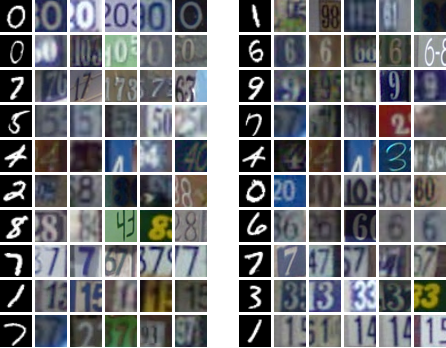
\includegraphics[width=\columnwidth]{digit_nn.png}
\caption{Example nearest neighbors for SVHN$\rightarrow$MNIST experiment. We show an example MNIST image and 5-NN SVHN images. Please note the large domain difference.}
\label{fig:nn}
\end{figure}

Table~\ref{tab:res} further suggests our algorithm significantly outperforms all state-of-the-art methods when there is large domain difference like MNIST$\leftrightarrow$MNIST-M, MNIST$\leftrightarrow$SVHN, Amazon$\leftrightarrow$Webcam and Amazon$\leftrightarrow$D-SLR. We hypothesize this performance is thanks to the transductive modeling. State-of-the-art algorithms like \cite{ganin15} are seeking for set of features invariant to the domains whereas we are seeking for an asymmetric similarity metric explaining both differences and similarities of two domains. In other words, instead of seeking for invariance, we seek for an equivariance. Specifically we seek for learning the exact transformation between two domains in the form of a similarity metric as well as a set of representative features.

\begin{figure}[ht]
\includegraphics[width=\columnwidth]{office_nn.png}
\caption{Example nearest neighbors for Amazon$\rightarrow$Webcam experiment. We show an example webcam image and 5-NN Amazon images. Please note the large domain difference.}
\label{fig:nn}
\end{figure}


Another interesting conclusion is the asymetric performance results. For example, the accuracy of adapting webcam images to amazon images and adapting amazon images to webcam images is significantly different. The similar behavior exist in MNIST and SVHN domains as well. This observation validates the importance of an asymetric modeling and the limited performance of domain invariance based methods since they are symmetric by definition. 

To further study the learned representations as well as the similarity metric, we perform a series of qualitative analysis in the form of nearest neighbor analysis and tSNE\cite{tsne} plots.

In Figure~\ref{fig:nn}, we visualize example target images from MNIST and their corresponding source images. First of all, both our experimental procedure and qualitative analysis suggests that MNIST and SVHN are the two domains with largest difference. Hence, we believe MNIST$\leftrightarrow$ is very challenging set-up. Moreover, our algorithm results in very accurate nearest neighbors.

The difference between invariance and equivariance is more clear in the tSNE plots of the office dataset in Figure~\ref{fig:tsne}. We plot same distribution twice with different color codings in Figure~\ref{fig:tsne}. In the first row, we color code the domain and the target and in the second row we color code object classes. The first observation is the effect of adaptation on the feature function. Clearly, the source domain is well clustered according to the object classes with and without adaptation. Moreover, this is expected since the features are specifically fine-tuned to the source domain. However, target domain has no structure. This is also expected since the algorithm did not see any target image. After the adaptation, target images also gets clustered according to the object classes. As comparison, we also visualize the tSNE plot of the domain invariant features obtained with \cite{ganin15}. Clearly, it is invariant to the domain however it is not discriminative since the loss function of \cite{ganin15} does not include any term for this purpose. We also draw lines between the nearest neighbor images of source and target images. 

\subsubsection{Effect of label propagation and feature learning}
\begin{figure}[ht]
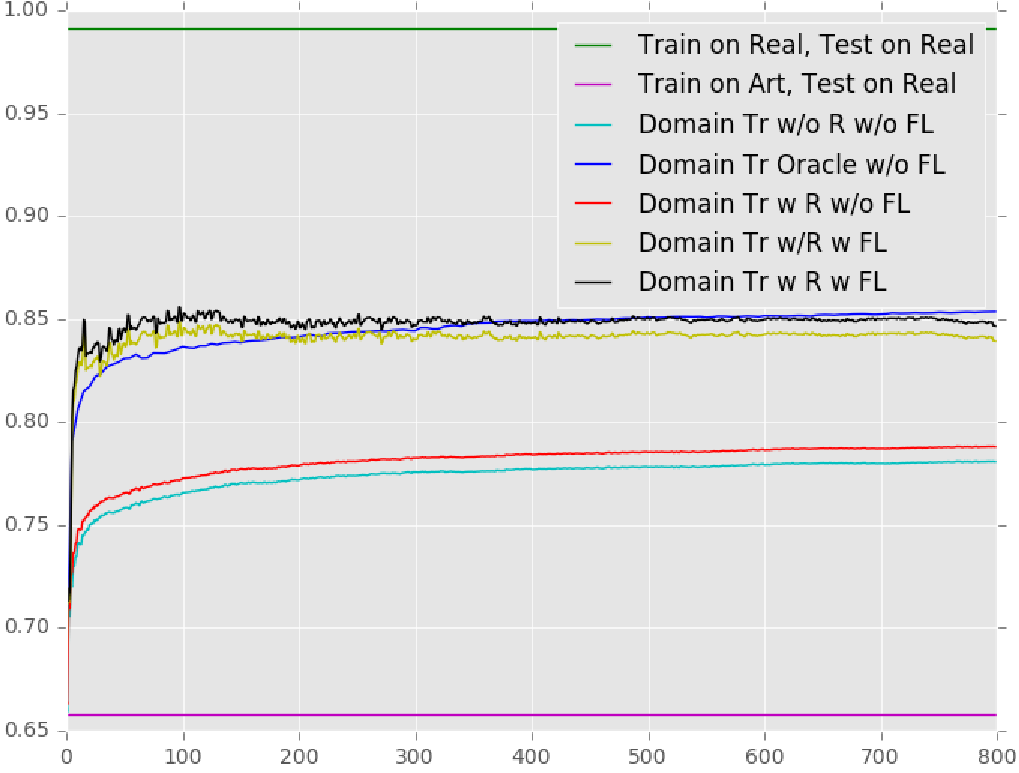
\includegraphics[width=\columnwidth]{figure_1fl}
\caption{Accuracy vs number of iterations for our-method, our-method-no-prop and our-method-no-fl. As the figure suggests the label propagation both increase the learning rate as well as the final accuracy. Moreover, the feature learning also have a significant effect on the accuracy.}
\label{fllprop}
\end{figure}
In order to evaluate the effect of having a robust label propagation and feature learning, we compare our method with a variant without the label propagation (noted as \emph{our-method-no-prop}) and a variant without feature learning (noted as \emph{our-method-no-fl}). We plot the accuracy vs number of iterations in order to evaluate both the effect on learning rate as well as the resultant accuracy. Although we plot the results only for MNIST$\rightarrow$MNIST-M, the other experiments have similar results and not displayed for the sake of clarity. Results are show in the Figure~\ref{fllprop}.  As the Figure~\ref{fllprop} suggests, both feature learning and label propagation is crucial for successful transduction. The feature learning has a slightly larger effect.

On the other hand, one interesting question is the effect of label propogation with respect to quality of the source only classifier. Clearly, when the source only classifier is accurate, label propogation has very limited effect. Hence, we re-train sub-optimal source only classifiers. Moreover, we show the performance of the over-all algorithm as well as the \emph{our-method-no-prop}. Moreover, we plot accuracy vs initialization (source only) quality in Figure~\ref{fig:init}. As figure~\ref{fig:init}, suggests the label propagation has very big when the initial classifier is not accurate. Moreover, overall algorithm is still accurate even when the initial source only classifier is sub-par.

\begin{figure*}[ht]
    \begin{subfigure}[b]{0.5\textwidth}
        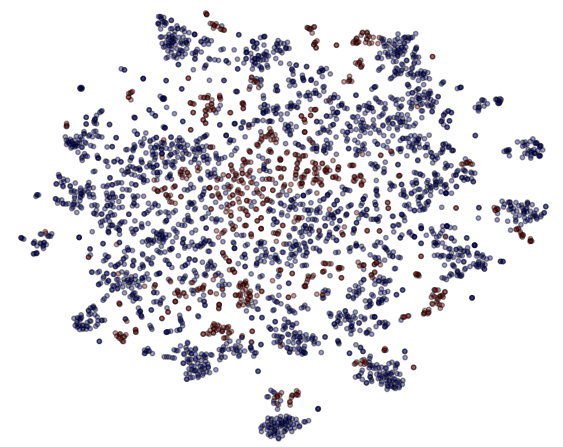
\includegraphics[width=\textwidth]{na_st.png}
        \caption{S. and T. w/o Adaptation}
        \label{fig:gull}
    \end{subfigure}~\begin{subfigure}[b]{0.5\textwidth}
        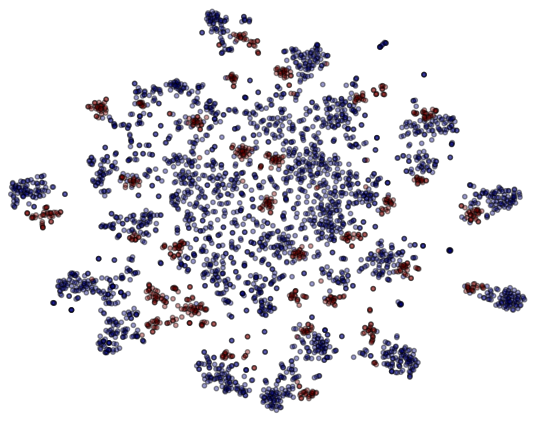
\includegraphics[width=\textwidth]{st.png}
        \caption{S. and T. with Adaptation}
    \end{subfigure}

    \begin{subfigure}[b]{0.5\textwidth}
        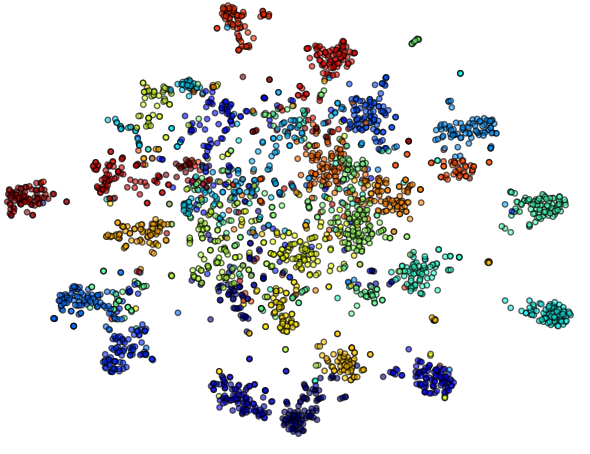
\includegraphics[width=\textwidth]{sc.png}
        \caption{Source Labels w/ Adaptation}
        \label{fig:gull}
    \end{subfigure}~\begin{subfigure}[b]{0.5\textwidth}
        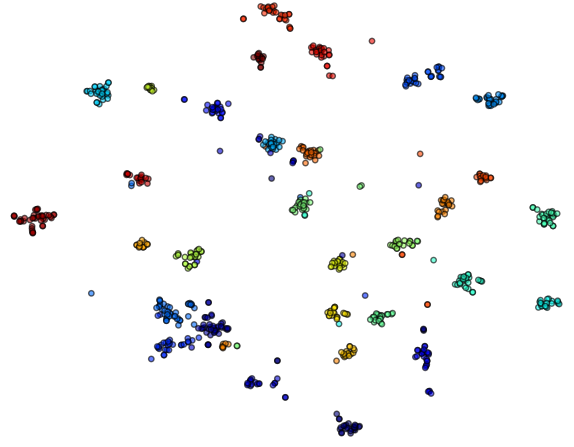
\includegraphics[width=\textwidth]{tc.png}
        \caption{Target Labels w/ Adaptation}
    \end{subfigure}
\caption{tSNE plots for features without and with unsupervised adaptation. Please note that the discriminative behavior emerges in the unsupervised target instead of source domain. This explain the motivation behind modeling the problem as transduction. In other words, our algorithm is designed to be accurate and discriminative in the target domain which is the domain we are interested in. Also note that our features are not invariant but the nearest neighbor arrows suggests that there is a consistent transformation, in other words our features are equivariant. }
\label{fig:tsne}
\end{figure*}

